\section{Introduction}
\label{sec:introduction}
Lightyear designs and develops solar electrice vehicles (SEVs), these are highly efficient battery powered vehicles that can charge their batteries using an integrated solar panel. The first vehicle designed by Lightyear is the \textit{Lightyear 0}, shown in Figure~\ref{fig:zero}.

\begin{figure}[htb]
    \centering
    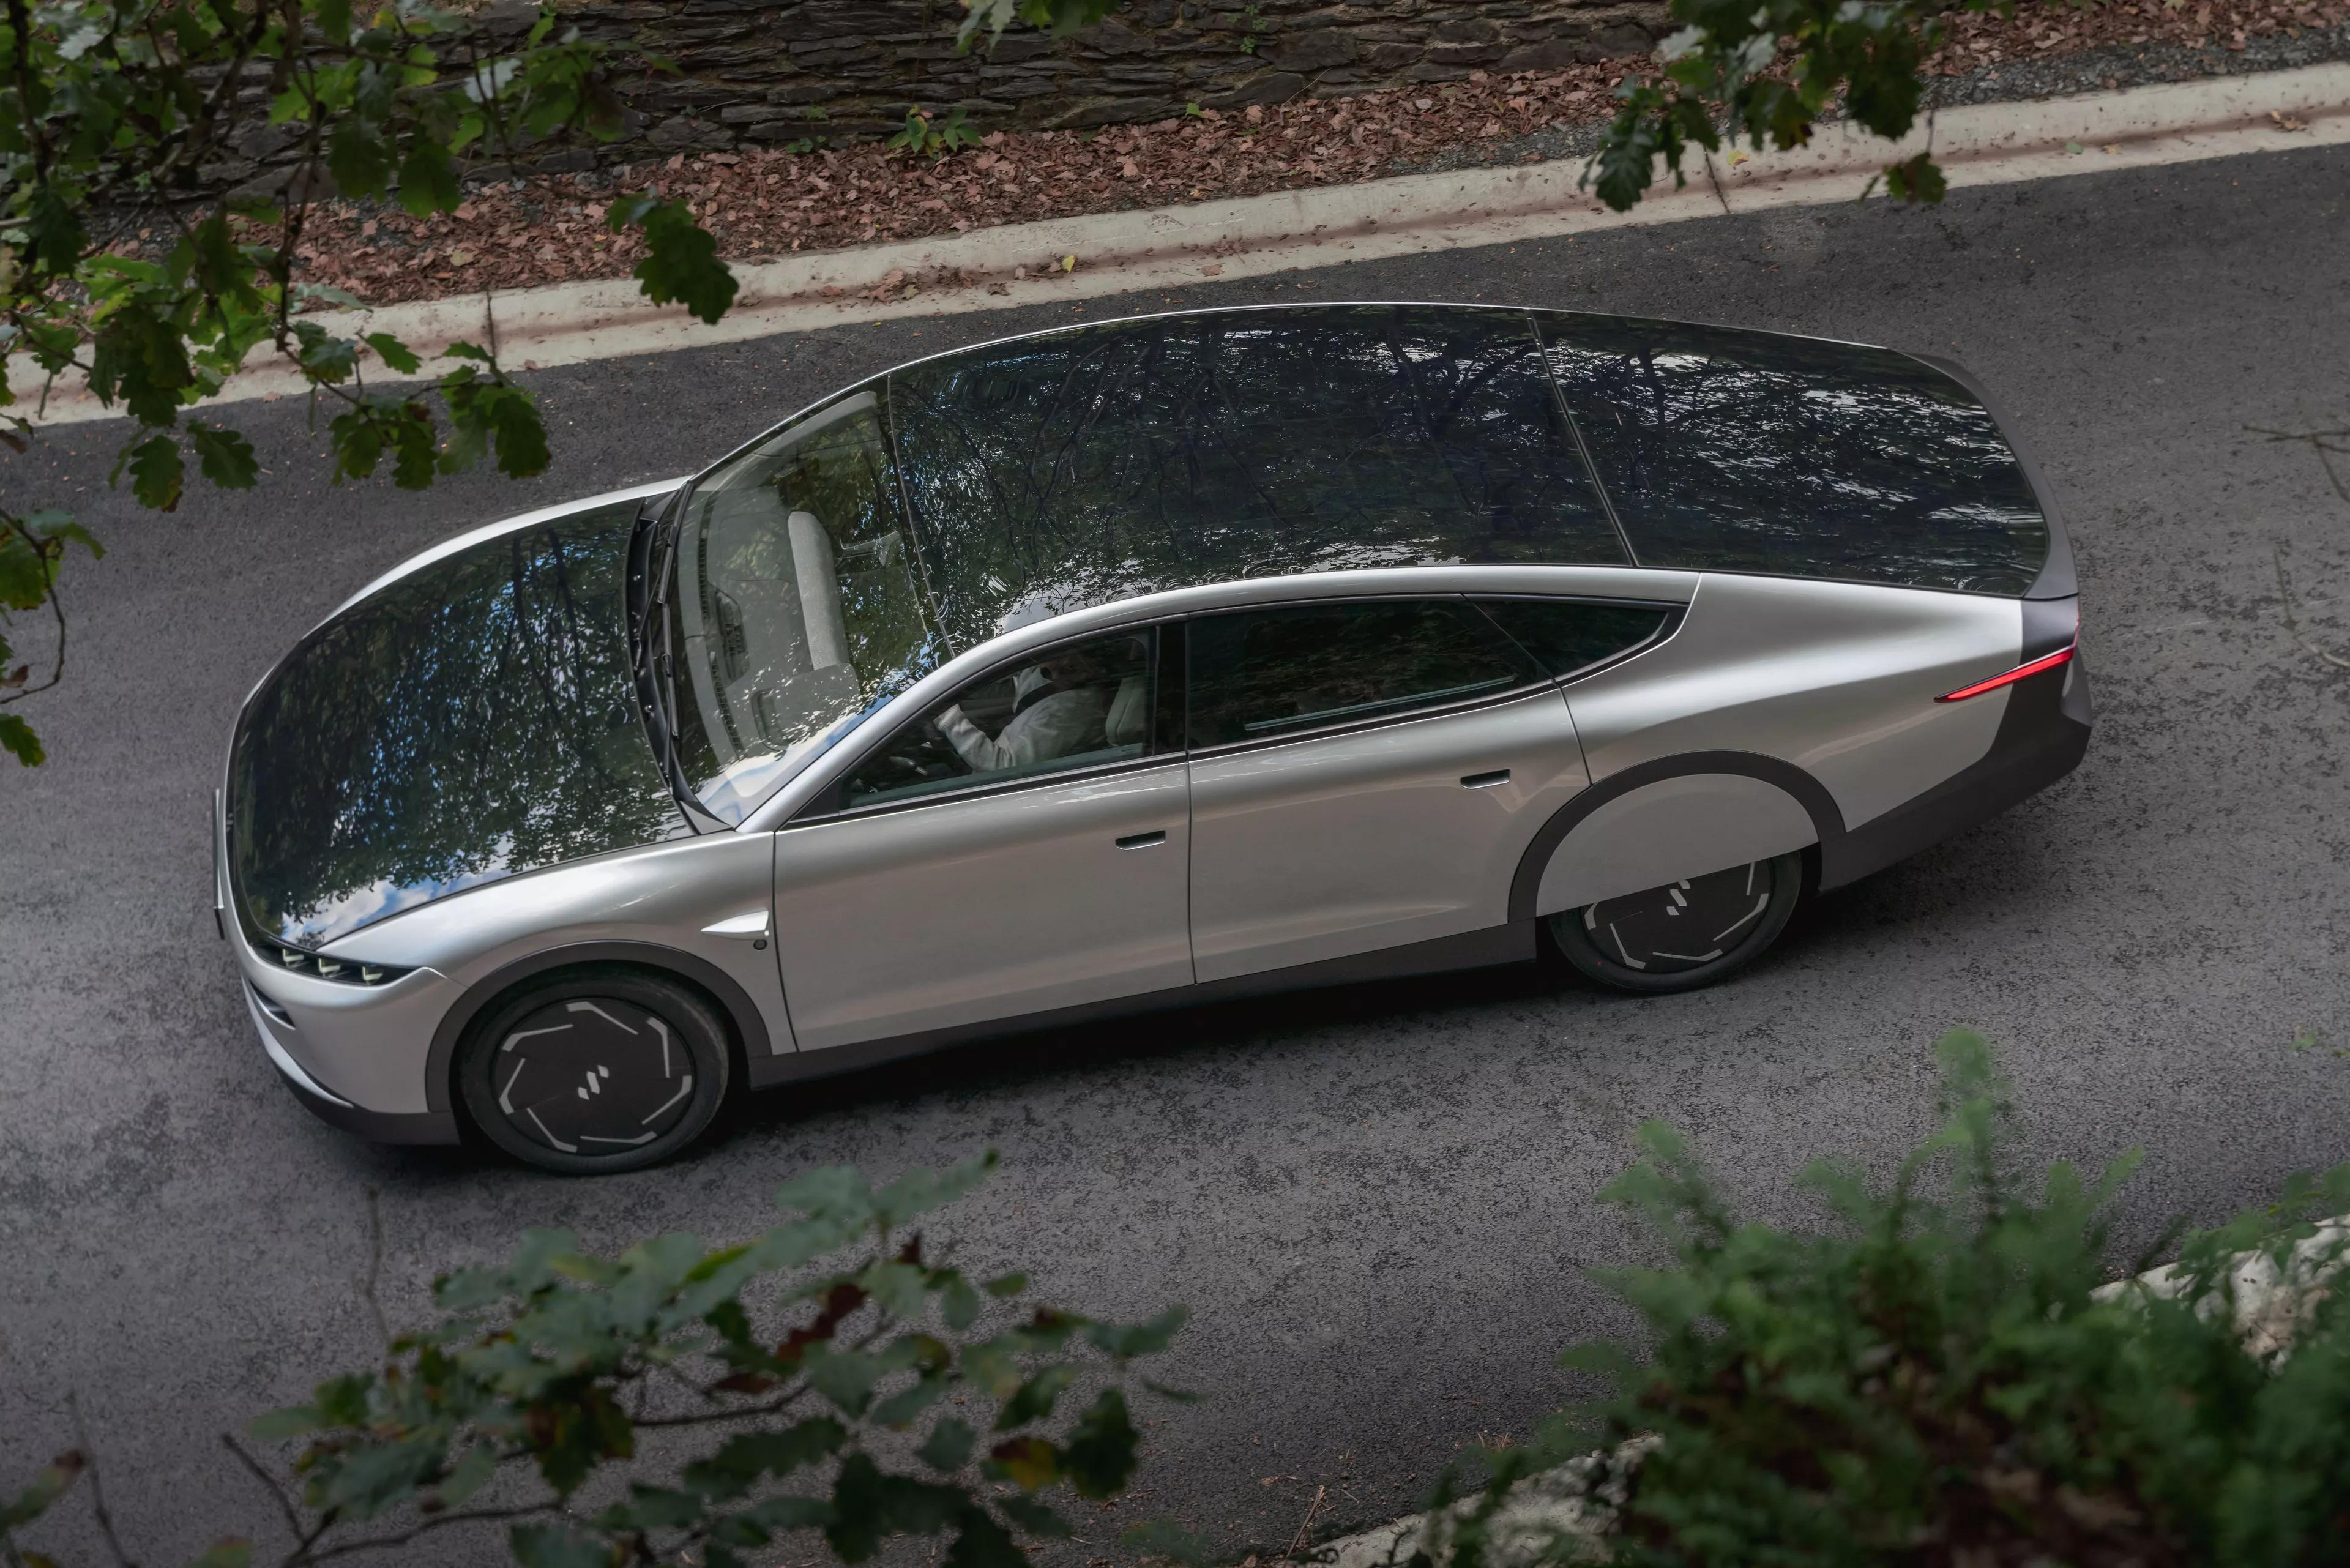
\includegraphics[width=0.9\textwidth]{images/Lightyear_zero.jpg}
    \caption{The Lightyear 0}
    \label{fig:zero}
\end{figure}

Some of the factors that play a role in a vehicle's efficiency are: aerodynamic drag, friction losses from tires, cabin heating and cooling, drivetrain losses and static energy consumption by the electric components. Lightyear seeks to design a vehicle that minimizes these losses as a reduction in energy consumption creates a positive feedback loop. For example, reducing the aerodynamic drag enables the use of a smaller battery while maintaining the same range. The smaller battery back reduces the vehicles weight, resulting in less friction losses from the tires, enabling the use of a smaller battery etc. Resulting in a vehicle with a very low energy consumption that can generate a significant amount of range from its integrated solar panels. One aspect which can be optimized is the weight and energy consumption of the electrical/electronic architecture.

\todo{Samenvatting van het onderzoek}
\todo{Structuur van het raport (sectie 2 ..., sectie 3 ...)}